\part{Docker}

\chapter{Под копотом}

\section{Из каких базовых вещей состоят контейнеры: namespaces, cgroups}
Все инструменты контейнеризации — будь то Docker, LXC или systemd-nspawn,— основываются на двух подсистемах ядра Linux: namespaces и cgroups. 

\subsection{chroot}

Идеи, лежащие в основе механизма пространств имён, не новы. Ещё в 1979 году в UNIX был добавлен системный вызов chroot() — как раз с целью обеспечить изоляцию и предоставить разработчикам отдельную от основной системы площадку для тестирования. 

Название chroot представляет собой сокращение от change root, что дословно переводится как «изменить корень». С помощью системного вызова chroot() и соответствующей команды можно изменить корневой каталог. Программе, запущенной с изменённым корневым каталогом, будут доступны только файлы, находящиеся в этом каталоге. 

Вершиной этой иерархии является каталог /, он же root. Все остальные каталоги — usr, local, bin и другие, — связаны с ним.

С помощью chroot в систему можно добавить второй корневой каталог, который с точки зрения пользователя ничем не будет отличаться от первого. Файловую систему, в которой присутствует изменённый корневой каталог, можно схематично представить на рис. \ref{3}.

\begin{figure}[h!]
\centering
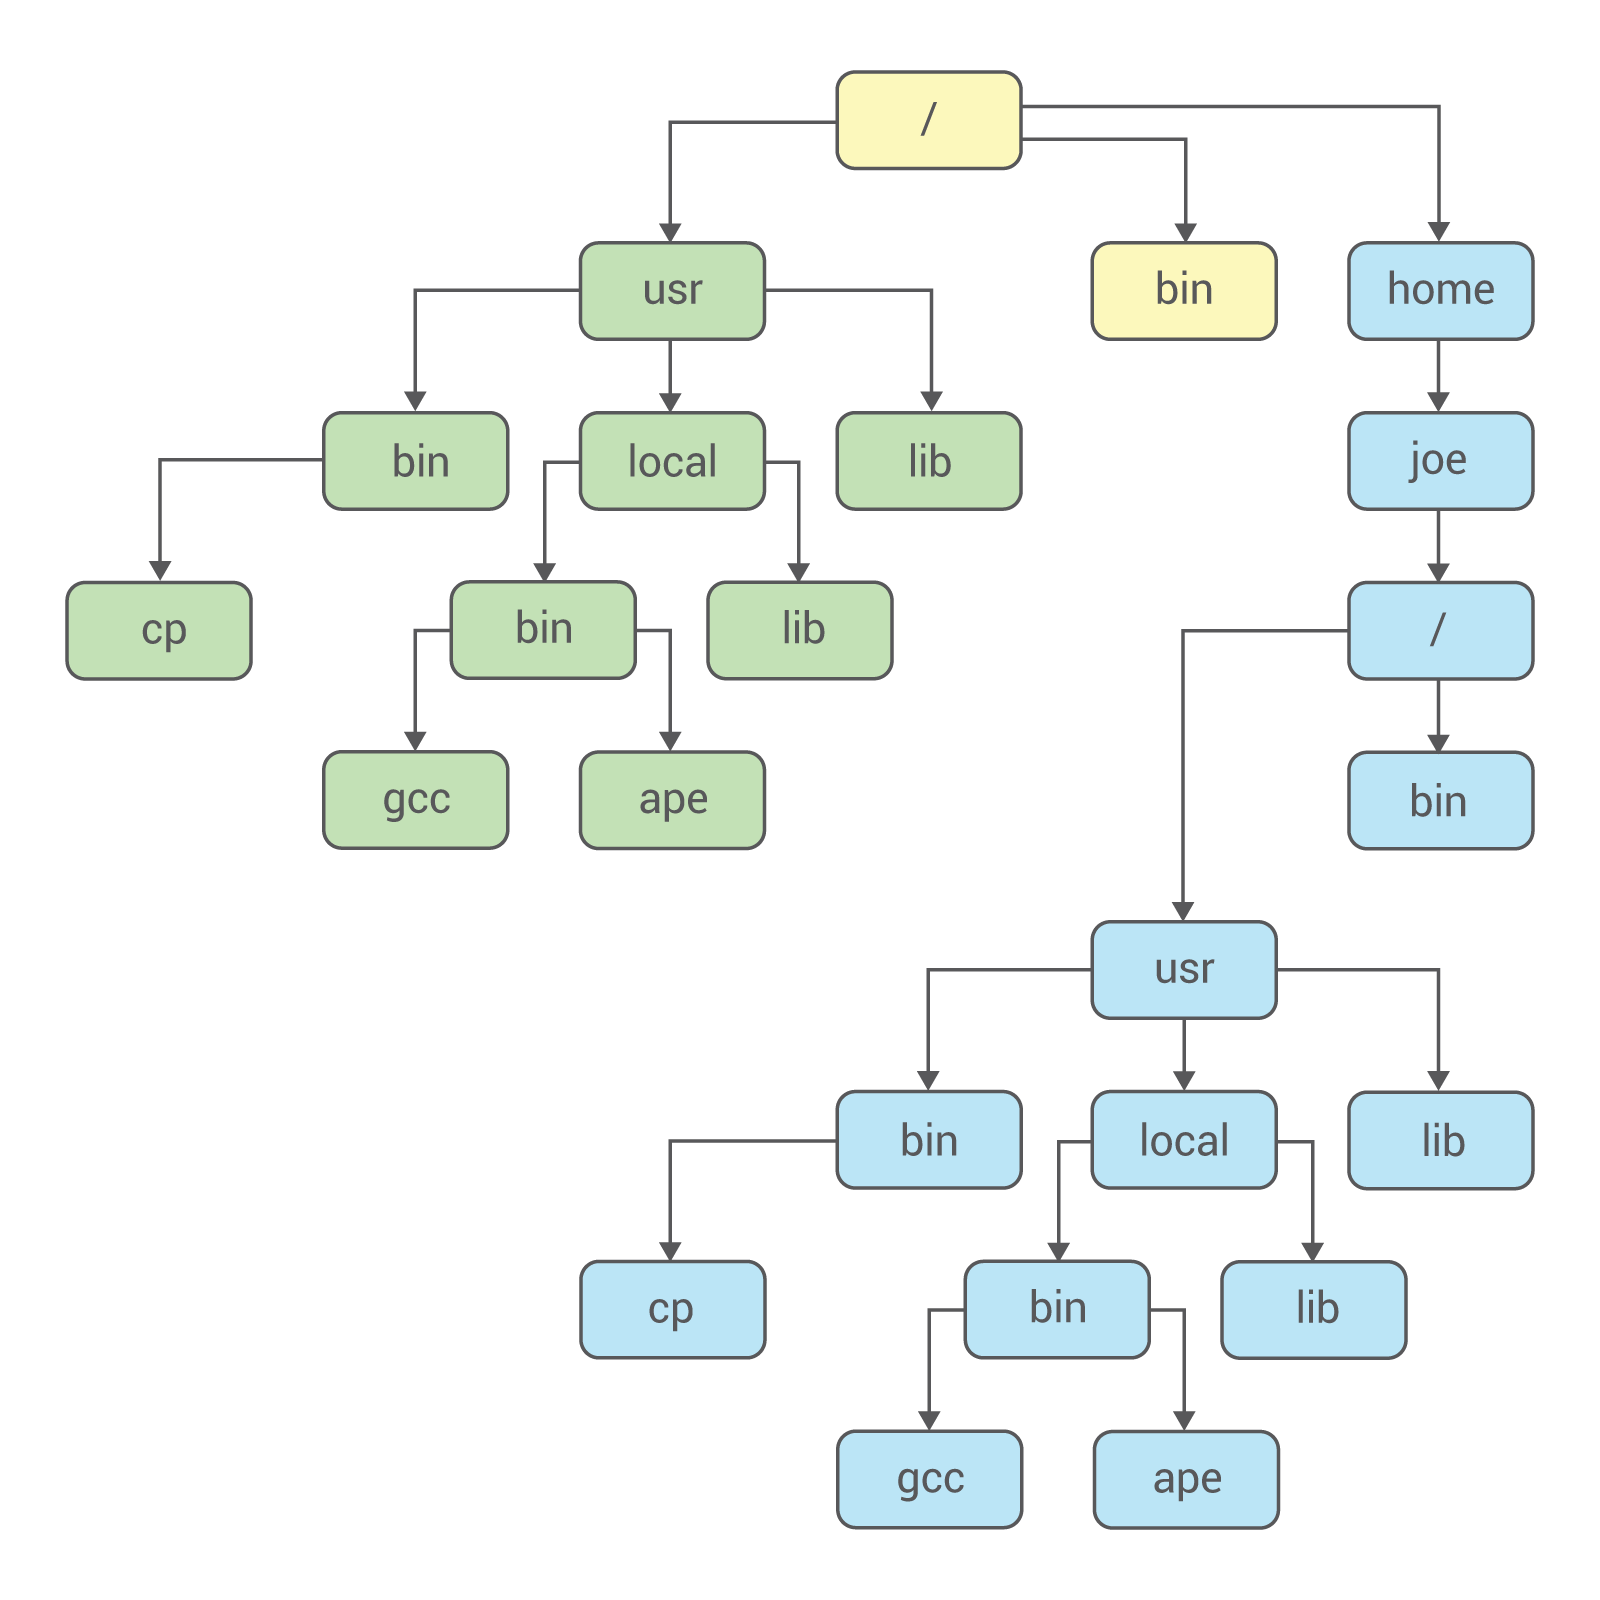
\includegraphics[width=0.9\textwidth]{chroot}
\caption{Представление файловой системы linux}
\label{fig3}
\end{figure}

\subsection{namespaces}

Пространство имён (англ. namespace) — это механизм ядра Linux, обеспечивающий изоляцию процессов друг от друга. Работа по его реализации была начата в версии ядра 2.4.19. На текущий момент в Linux поддерживается шесть типов пространств имён:

\begin{table}[]
\begin{tabular}{|l|l|}
\hline
Пространство имен & Что изолирует  \\ \hline
PID & PID процессов  \\ \hline
NETWORK & Сетевые устройства, стеки, порты... \\ \hline
USER & ID пользователей и групп \\ \hline
MOUNT & Точки монтирования \\ \hline
IPC & SystemV IPC, очереди сообщений POSIX \\ \hline
UTS & Имя хоста и доменное имя NIS \\ \hline
\end{tabular}
\end{table}

Неймспейсы изолируют друг от другая процессы таким образом, что процессы в одной группе не могут видеть ресурсы другой группы. Например, PID namespace предоставляет уникальные идентификаторы процессов в рамках группы. Внутри одной группы может быть процесс с pid 1 и внутри второй группы тоже может быть процесс с pid 1, хотя это два совершенно разных процесса, которые друг о другие ничего не знают. Притом, все процессы все также имеют уникальные id в рамках ОС. Просто, если смотреть на процессы из группы, то эти id отображаются в другие.

\subsubsection{PID: изоляция PID процессов}

При загрузке в Linux сначала запускается процесс с идентификационным номером (PID) 1. В дереве процессов он является корневым. Он запускает другие процессы и службы. Механизм namespaces позволяет создавать отдельное ответвление дерева процессов с собственным PID 1. Процесс, который создаёт такое ответвление, являются частью основного дерева, но его дочерний процесс уже будет корневым в новом дереве.

Процессы в новом дереве никак не взаимодействуют с родительским процессом и даже не «видят» его. В то же время процессам в основном дереве доступны все процессы дочернего дерева. Наглядно это показано на рис.

\begin{figure}[h!]
\centering
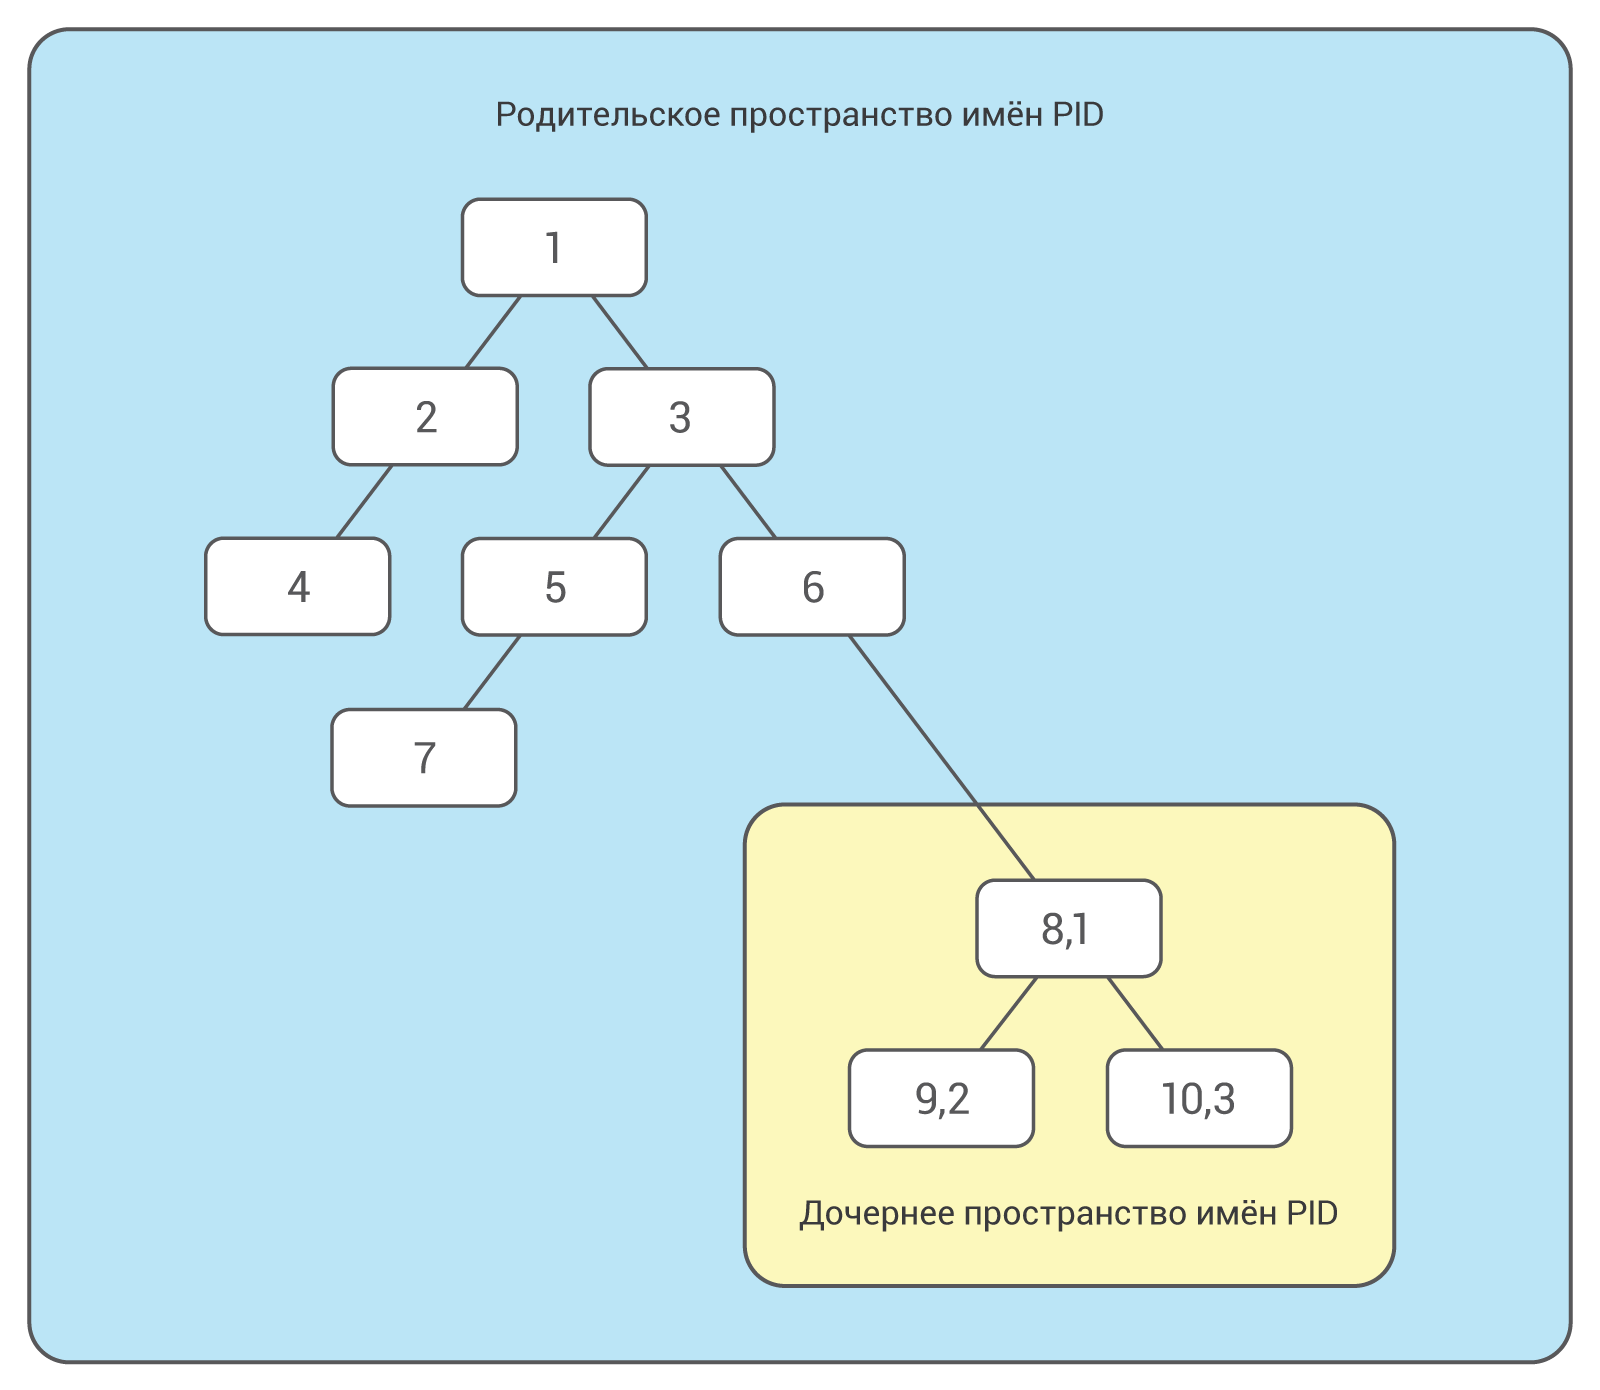
\includegraphics[width=0.9\textwidth]{pid}
\caption{Представление файловой системы linux}
\label{fig4}
\end{figure}

\subsubsection{NET: изоляция сетей}

Благодаря пространству имён NET мы можем выделять для изолированных процессов собственные сeтевые интерфейсы. Даже loopback-интерфейс для каждого пространства имён будет отдельным.

Сетевые пространства имён можно создавать с помощью системного вызова clone() с флагом CLONE\_NEWNET. 

\subsubsection{MOUNT: изоляция файловой системы}

Об изоляции на уровне файловой системы мы уже упоминали выше, когда разбирали системный вызов chroot (). Мы отметили, что системный вызов chroot() не обеспечивает надёжной изоляции. С помощью же пространств имён MOUNT можно создавать полностью независимые файловые системы, ассоциируемые с различными процессами.

\subsection{cgroups (Control Groups)}

Позволяют организовывать процессы в группы и для каждой группы задавать лимиты. Например, лимиты на использование CPU, объем используемой памяти и дисковый ввод-вывод.

Механизм cgroups состоит из двух составных частей: ядра (cgroup core) и так называемых подсистем. В ядре версии 4.4.0.21 таких подсистем 12:

\begin{itemize}
\item blkio — устанавливает лимиты на чтение и запись с блочных устройств;
\item cpuacct — генерирует отчёты об использовании ресурсов процессора;
\item cpu — обеспечивает доступ процессов в рамках контрольной группы к CPU;
\item cpuset — распределяет задачи в рамках контрольной группы между процессорными ядрами;
\item devices — разрешает или блокирует доступ к устройствам;
\item freezer — приостанавливает и возобновляет выполнение задач в рамках контрольной группы
\item hugetlb — активирует поддержку больших страниц памяти для контрольных групп;
\item memory — управляет выделением памяти для групп процессов;
\item net\_cls — помечает сетевые пакеты специальным тэгом, что позволяет идентифицировать пакеты, порождаемые определённой задачей в рамках контрольной группы;
\item netprio — используется для динамической установки приоритетов по трафику;
\item pids — используется для ограничения количества процессов в рамках контрольной группы.
\end{itemize}

Каждая подсистема представляет собой директорию с управляющими файлами, в которых прописываются все настройки.  

\subsection{Отличия namespaces от cgroups}

\textbf{cgroup}: Контрольные группы предоставляют механизм для агрегирования или разбиения наборов задач и всех их будущих детей в иерархические группы со специализированным поведением.
\textbf{namespace}: обертывает глобальный системный ресурс в абстракции, которая заставляет его казаться процессам в пространстве имен, что у них есть свой отдельный экземпляр глобального ресурса.

\textbf{Вкратце}:

 cgroups = ограничивает, сколько вы можете использовать;
 namespaces = пределы того, что вы можете видеть (и, следовательно, использовать)

\section{Как docker прокидывает порт}

\chapter{Шпаргалка}

Полезная \href{https://docs.docker.com/engine/reference/builder/#usage}{ссылка} на документацию по основным операторам Dockerfile.

\subsection{ENV}

Пример использования в Dockerfile:
\begin{lstlisting}
ENV EDITOR 
\end{lstlisting}

\subsection{ARG}

Сборка с использованием аргументов, указать строку в Dockerfile:
\begin{lstlisting}
ARG UID
\end{lstlisting}

Аргументы по-умолчанию:
\begin{lstlisting}
ARG UID=1000
\end{lstlisting}

При сборке использовать параметр:
\begin{lstlisting}
docker build --build-arg UID=what_user .
\end{lstlisting}

\subsection{USER}

Специфицирует пользователя, под которым должен быть запущен образ. Мы можем указать имя пользователя или UID и группу или GID. Варианты использования команды:
\begin{lstlisting}
USER user
USER user:group
USER uid
USER uid:gid
USER user:gid
USER uid:group
\end{lstlisting}
Вы можете перегрузить эту команду, используя флаг -u при запуске контейнера. Если пользователь не указан, используется root по-умолчанию.

Пример конфигурирования пользователя при сборке, получая аргументом по-умолчанию UID: 
\begin{lstlisting}
ARG UID=1000
USER $UID
\end{lstlisting}

Сборка контейнера с заданием UID:
\begin{lstlisting}
docker build -t dockerfile-extended --build-arg UID=1001 .
\end{lstlisting}

\subsection{WORKDIR}

Создание и установка рабочей директории по-умолчанию:
\begin{lstlisting}
WORKDIR /home/stepik
\end{lstlisting}
Вы можете перегрузить рабочую директорию контейнера в рантайме с помощью флага -w.

\subsection{CMD и ENTRYPOINT}

The CMD instruction has three forms:
\begin{itemize}
\item CMD ["executable","param1","param2"] (exec form, this is the preferred form)
\item CMD ["param1","param2"] (as default parameters to ENTRYPOINT)
\item CMD command param1 param2 (shell form)
\end{itemize}

Это значит контейнеры собранные из этих файлов выводят одинаковую информацию:


\begin{itemize}
\item Без определения ENTRYPOINT:
\begin{lstlisting}
FROM ubuntu:latest
CMD ["printf", "Hello %s!\n", "World"]
\end{lstlisting}
\item С определением ENTRYPOINT:
\begin{lstlisting}
FROM ubuntu:latest
ENTRYPOINT ["printf"]
CMD ["Hello %s!\n", "World"]
\end{lstlisting}
\end{itemize}

\subsection{Передача параметров в контейнер}
Если быть точным, то это переопределение параметров запуска контейнера.
Если создать контейнер из файла:
\begin{lstlisting}
FROM ubuntu
ENTRYPOINT ["printf", "Hello %s!\n"]
CMD ["World"]
\end{lstlisting}
И запустить его командой:
\begin{lstlisting}
docker run --rm test
\end{lstlisting}
То вывод будет:
\begin{lstlisting}
Hello World!
\end{lstlisting}

Если изменить команду запуска:
\begin{lstlisting}
docker run --rm test John
\end{lstlisting}
То вывод будет:
\begin{lstlisting}
Hello John!
\end{lstlisting}


\section{ps}

\subsection{Просмотр работающих контейнеров}
\begin{lstlisting}
docker ps
\end{lstlisting}

\subsection{Просмотр всех контейнеров}
\begin{lstlisting}
docker ps -a
\end{lstlisting}

\section{run}

\subsection{Создание и запуск контейнера}
\begin{lstlisting}
docker run --rm -it --name new_name debian:latest bash
\end{lstlisting}

\begin{enumerate}
\item \textbf{--rm} - удалить контейнер после остановки.
\item \textbf{-it} - interactive tty, подключение к интерактивной консоли, в данном случае запуск bash.
\item \textbf{--name} - задаем имя контейнеру, в данном случае: new\_name.
\item \textbf{debian:latest} - обязательный параметр, образ от которого наследуемся.
\end{enumerate}

\subsection{Создание контейнера, который стартует при загрузке системы}
\begin{lstlisting}
docker run -d --restart=always debian:latest
\end{lstlisting}
\begin{enumerate}
\item \textbf{-d} - detach mode, если в контейнере есть "ожидающий или слушающий" процесс, то конейнер не завершится, пока его не попросить.
\item \textbf{--restart} - с параметром \textit{always} конейнер стартует сам.
\end{enumerate}

\subsection{Монтирование постоянного хранилища}
\begin{lstlisting}
docker run -d -v my_data:/etc/nginx/ debian:latest
\end{lstlisting}
Имя хранилища - \textit{my\_data}

\subsection{Монтирование постоянного папки хоста}
\begin{lstlisting}
docker run -d -v /var/log/nginx/:/tmp/logs/nginx/ debian:latest
\end{lstlisting}
\begin{itemize}
\item Имя папки хоста: /var/log/nginx/
\item Имя папки контейнера: /tmp/logs/nginx/
\end{itemize}


\subsection{Проброс порта}
\begin{lstlisting}
docker run -d -p 3344:80 debian:latest
\end{lstlisting}
\begin{itemize}
\item Номер внешнего порта хоста, доступный из сети: 3344
\item Номер порта контейнера доступный только из виртуальной сети docker: 80
\end{itemize}

\section{exec}
Подключение к уже работающему контейнеру:
\begin{lstlisting}
#Lets run bash from work container name 'worked_container':
docker exec -it worked_container bash
\end{lstlisting}

\section{volume}
\subsection{Создание хранилища для постоянных данных}
\begin{lstlisting}
docker volume create my_data
\end{lstlisting}

\subsection{Список осиротевших томов}
\begin{lstlisting}
docker volume ls -qf dangling=true
\end{lstlisting}


\section{network}
\section{commit}
Создание образа с изменением его точки входа:
\begin{lstlisting}
#Container create
docker run -it --name create-image-from-me ubuntu:14.04 /bin/true
#Lets change container and set new entry point:
docker commit --change='ENTRYPOINT ["/usr/bin/python3"]' create-image-from-me my-python:latest
#my-python:latest - new image name and tag
#Lets run new container from new image
docker run --rm -it my-python:latest
\end{lstlisting}



\section{build}

\subsection{Пример Dockerfile}

\lstinputlisting{Dockerfile1.txt}

\subsection{Сборка образа из Dockerfile}
\begin{lstlisting}
docker build -t myimage -f Dockerfile .
\end{lstlisting}
\begin{itemize}
\item \textbf{-t} - параметр определяющий имя нового образа.
\item \textit{-f} - задание Dockerfile не по-умолчанию, не обязательный параметр..
\item \textbf{.} - задание директории для сборки, в данном случае это будет текущая директория. Обязательный параметр.
\end{itemize}


\section{Полезные команды}
\subsection{Удалить все образы, не помеченные тегами}
\begin{lstlisting}
docker rmi $(docker images | grep '^<none>' | awk '{print $3}')
docker rmi $(docker images -f "dangling=true" -q)
\end{lstlisting}
